\include{preamble}






\begin{document}
  \maketitle

%\includegraphics[scale=0.55]{frontpage}

  \section{Results}

  The following table summarizes our result:
  
    \bigskip\noindent
  \begin{tabular}{lr}
  	\toprule
  	Input file & MST total weight \\ \midrule
  	USA-highway-miles.txt	 & 16598.0 \\
  	tinyEWG-alpha.txt & 181 \\ \bottomrule
  \end{tabular}
  
    \bigskip
  
     The MST we found in tinyEWG-alpha.txt can be drawn like this:
     
     
     
     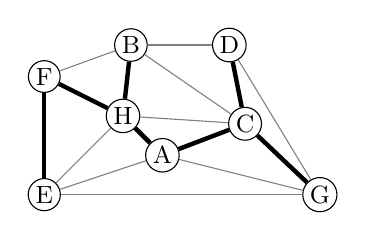
\begin{tikzpicture}[
     scale = .5,
     every node/.style = {
     	circle, draw, black, inner sep = 1pt, font = \small},
     every path/.style = {gray}
     ]
     
       \node (A) at (3,1) {A}; % 0
       \node (B) at (2.2,3.8) {B}; % 1
       \node (C) at (5.1,1.8) {C}; % 2
       \node (D) at (4.7,3.8) {D}; % 3
       \node (E) at (0,0) {E}; % 4
       \node (F) at (0,3) {F}; % 5
       \node (G) at (7,0) {G}; % 6
       \node (H) at (2,2) {H}; % 7
       \draw (E)--(F);
       \draw (E)--(H);
       \draw (F)--(H);
       \draw (A)--(H);
       \draw (B)--(F);
       \draw (A)--(E);
       \draw (C)--(D);
       \draw (B)--(H);
       \draw (A)--(C);
       \draw (B)--(C);
       \draw (B)--(D);
       \draw (C)--(H);
       \draw (G)--(C);
       \draw (D)--(G);
       \draw (G)--(A);
       \draw (G)--(E);
       \begin{scope}[every path/.style={ultra thick}]
       \draw(A)--(H);
       \draw(B)--(H);
       \draw(A)--(C);
       \draw(C)--(D);
       \draw(F)--(H);
       \draw(E)--(F);
       \draw(G)--(C);
       \end{scope}
     
     
     
     
      \end{tikzpicture}
      
  
  
  The MST has the following edges (lenghts in drawing are not correct):
  
  A - H weight: 16.0
  
  B - H weight: 19.0
  
  A - C weight: 26.0
  
  C - D weight: 17.0
  
  F - H weight: 28.0
  
  E - F weight: 35.0
  
  G - C weight: 40.0
  
  Total lenght of MST: 181.0 
  
  \section{Implementation details}

  We implemented the algorithms from the book page: 
  
  LazyPrimMST.java using MinPQ.java. The total running time is E*log(E) in worst case for Prim.
  
  To this should be added the time to create the graph - not considering the time it takes to remove white space this takes V+E (the number of lines in the file). 
  
  
  
  

\end{document}
